% filepath: /Users/donny/Documents/GitHub/computer-vision/Tikz/image-videos/convolution.tex

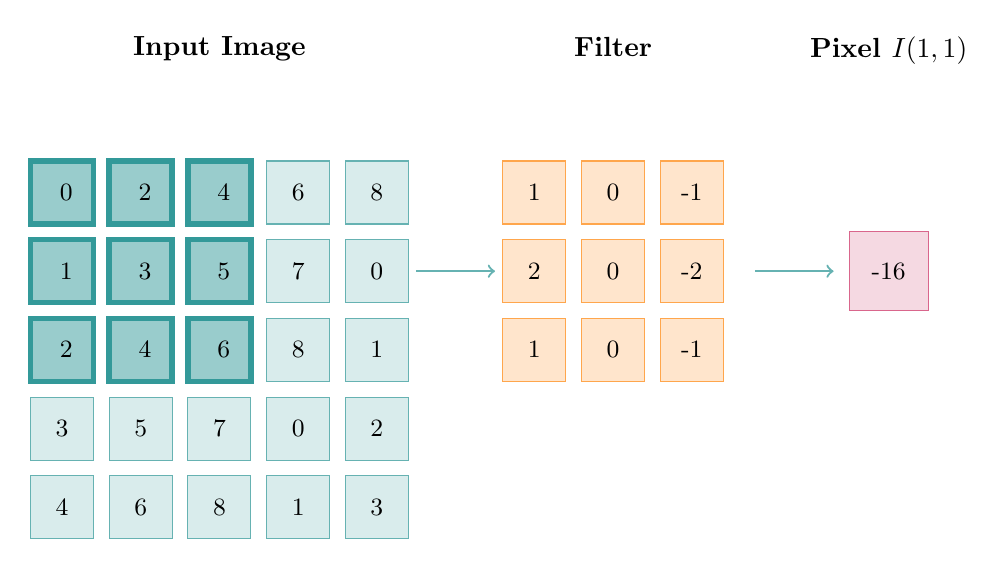
\begin{tikzpicture}[
    cell/.style={draw, rectangle, minimum width=0.8cm, minimum height=0.8cm, font=\small},
    cell-input/.style={cell, fill=teal!15, draw=teal!60},
    cell-highlight/.style={cell, fill=teal!40, draw=teal!80, line width=2pt},
    cell-kernel/.style={cell, fill=orange!20, draw=orange!70},
    cell-output/.style={cell, fill=purple!15, draw=purple!60, minimum width=1cm, minimum height=1cm},
    arrow/.style={->, thick, color=teal!60},
    label/.style={font=\normalsize, font=\bfseries}
]

% --- Input Image Grid (5x5) ---
\node[label, below=0.4cm] at (2, 2.5) {Input Image};
\foreach \i in {0,1,2,3,4} {
    \foreach \j in {0,1,2,3,4} {
        \pgfmathtruncatemacro{\val}{int(mod(\i + 2*\j, 9))}
        \node[cell-input] at (\j,-\i) {\val};
    }
}

% Highlight 3x3 region (top-left 3x3)
\foreach \i in {0,1,2} {
    \foreach \j in {0,1,2} {
        \node[cell-highlight] at (\j,-\i) {
            \pgfmathtruncatemacro{\val}{int(mod(\i + 2*\j, 9))}
            \val
        };
    }
}

% --- Kernel (3x3) ---
\node[label, below=0.4cm] at (7, 2.5) {Filter};
\node[cell-kernel] at (6, 0) {1};
\node[cell-kernel] at (7, 0) {0};
\node[cell-kernel] at (8, 0) {-1};

\node[cell-kernel] at (6, -1) {2};
\node[cell-kernel] at (7, -1) {0};
\node[cell-kernel] at (8, -1) {-2};

\node[cell-kernel] at (6, -2) {1};
\node[cell-kernel] at (7, -2) {0};
\node[cell-kernel] at (8, -2) {-1};

% --- Arrow ---
\draw[arrow] (4.5,-1) -- (5.5,-1);
\draw[arrow] (8.8,-1) -- (9.8,-1);
% --- Output ---
\node[label, below=0.4cm] at (10.5, 2.5) {Pixel $I(1,1)$};
\node[cell-output] at (10.5, -1) {-16};

\end{tikzpicture}